\begin{prob}
    Suppose a BFS is run on the graph below using node 1 as the source node. Which
    node will be the BFS predecessor of node 9? You should use the convention that neighbors
    are produced in ascending order by label.


    \begin{center}
        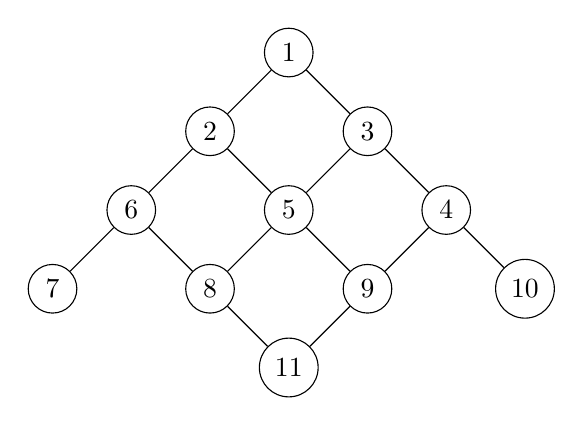
\begin{tikzpicture}
            {
                \tikzset{every node/.style = {shape=circle, draw, minimum size=17pt}}

                \node (1) at (0, 0) {$1$};
                \node (2) at (-1, -1) {$2$};
                \node (3) at (1, -1) {$3$};
                \node (4) at (2, -2) {$4$};
                \node (5) at (0, -2) {$5$};
                \node (6) at (-2, -2) {$6$};
                \node (7) at (-3, -3) {$7$};
                \node (8) at (-1, -3) {$8$};
                \node (9) at (1, -3) {$9$};
                \node (10) at (3, -3) {$10$};
                \node (11) at (0, -4) {$11$};
            }

            
            \draw (1) edge[-]  (2);
            \draw (1) edge[-]  (3);
            \draw (2) edge[-]  (6);
            \draw (2) edge[-]  (5);
            \draw (3) edge[-]  (5);
            \draw (3) edge[-]  (4);
            \draw (6) edge[-]  (7);
            \draw (6) edge[-]  (8);
            \draw (5) edge[-]  (8);
            \draw (5) edge[-]  (9);
            \draw (4) edge[-]  (9);
            \draw (4) edge[-]  (10);
            \draw (8) edge[-]  (11);
            \draw (9) edge[-]  (11);

        \end{tikzpicture}
    \end{center}
    

    \inlineresponsebox[.75in]{5}

\end{prob}
